\documentclass[a4paper,12pt,abstracton]{scrartcl}
\usepackage[utf8]{inputenc}
\usepackage{float}
\usepackage{tikz}
\usepackage{amsmath}
\usepackage{amssymb}
\usepackage{pifont}% http://ctan.org/pkg/pifont
\usepackage[font=small,labelfont=bf]{caption}
\usepackage{graphicx}
\usepackage{dirtytalk}
\usepackage{multicol}
\usepackage{booktabs}
\usepackage{colortbl}
\usepackage{appendix}
\usepackage{nomencl}
\usepackage{lmodern}
\usepackage[nottoc]{tocbibind}
\usepackage{xcolor}
%\graphicspath{images/}
\usepackage[margin = 3cm]{geometry}
\usepackage{ragged2e} % good alignment
\usepackage{hyperref}
\usepackage{siunitx} % Provides the \SI{}{} and \si{} command for typesetting SI units
\hypersetup{colorlinks=true,
    linkcolor=blue,
    filecolor=magenta,      
    urlcolor=cyan, 
    citecolor=gray}

%\DeclareGraphicsExtensions{.png,.pdf} % low-res (work in progress)
%\DeclareGraphicsExtensions{.pdf,.png}  % high-res (final draft)
%\setlength\parindent{0pt} % Removes all indentation from paragraphs
%\bibliographystyle{unstr}
\setlength\parindent{0pt}
\setlength{\parskip}{0.3em}
\newcommand{\xmark}{\ding{55}}

\renewcommand{\nomname}{List of Symbols}
\renewcommand{\nompreamble}{The following list explains the symbols used within the body of the report.}

\usepackage{etoolbox}
\renewcommand\nomgroup[1]{%
  \item[\bfseries
  \ifstrequal{#1}{E}{Experimental Equipment}{%
  \ifstrequal{#1}{C}{Computational Methods}{%
  \ifstrequal{#1}{T}{Theoretical Concepts}{
  \ifstrequal{#1}{P}{Physical Constants}{}}}}%
]}

\begin{document}
\section{Calibration}\label{sec:cal}

\subsection{Data Collection}
In order to calibrate the magnet it is necessary to establish the dependence of the magnetic field $B$ from the current $I$ injected in the coils. Therefore we gradually increased and then decreased $I$ as shown in \hyperref[table:BI1]{Table \ref*{table:BI1}}  and \hyperref[table:BI2]{ \ref*{table:BI2}} respectively. 

\begin{table}[H]
\centering
\caption{}
\label{table:BI1}
\begin{tabular}{c c}
\addlinespace
\addlinespace
\resizebox{6cm}{!}{
\begin{tabular}{cc}
\toprule
$I\;[A]$ & $B\;[T]$\\
\midrule
 0.00 $\pm$ 0.02 & 0.000 $\pm$ 0.001\\
 1.02 $\pm$ 0.02 & 0.071 $\pm$ 0.001\\
  2.03 $\pm$ 0.02 & 0.140 $\pm$ 0.001\\
 3.00 $\pm$ 0.02 & 0.205 $\pm$ 0.001\\
  4.04 $\pm$ 0.02 & 0.277 $\pm$ 0.001\\
4.99 $\pm$ 0.02 & 0.342 $\pm$ 0.001\\
  6.02 $\pm$ 0.02 & 0.408 $\pm$ 0.001\\
7.00 $\pm$ 0.02 & 0.471 $\pm$ 0.001\\
  8.02 $\pm$ 0.02 & 0.535 $\pm$ 0.001\\
8.48 $\pm$ 0.02 & 0.563 $\pm$ 0.001\\
 9.01 $\pm$ 0.02 & 0.588 $\pm$ 0.001\\
9.51 $\pm$ 0.02 & 0.612 $\pm$ 0.001\\
 10.04 $\pm$ 0.02 & 0.636 $\pm$ 0.001\\
\bottomrule
\end{tabular}}
\hspace{2cm}
\resizebox{6cm}{!}{
\begin{tabular}{cc}
\toprule
$I\;[A]$ & $B\;[T]$\\
\midrule
  10.04 $\pm$ 0.02 & 0.636 $\pm$ 0.001\\
 9.50 $\pm$ 0.02 & 0.613 $\pm$ 0.001\\
8.97 $\pm$ 0.02 & 0.590 $\pm$ 0.001\\
 8.49 $\pm$ 0.02 & 0.566 $\pm$ 0.001\\
7.00 $\pm$ 0.02 & 0.478 $\pm$ 0.001\\
  6.05 $\pm$ 0.02 & 0.416 $\pm$ 0.001\\
4.98 $\pm$ 0.02 & 0.348 $\pm$ 0.001\\
 4.02 $\pm$ 0.02 & 0.282 $\pm$ 0.001\\
3.00 $\pm$ 0.02 & 0.215 $\pm$ 0.001\\
 2.00 $\pm$ 0.02 & 0.145 $\pm$ 0.001\\
1.00 $\pm$ 0.02 & 0.078 $\pm$ 0.001\\
 0.00 $\pm$ 0.02 & 0.009 $\pm$ 0.001\\
\\
\bottomrule
\end{tabular}}
\end{tabular}
\end{table}
\begin{table}[H]
\centering
\caption{}
\label{table:BI2}
\begin{tabular}{c c}
\addlinespace
\addlinespace
\resizebox{6cm}{!}{
\begin{tabular}{cc}
\toprule
$I\;[A]$ & $B\;[T]$\\
\midrule
 0.00 $\pm$ 0.02 & 0.009 $\pm$ 0.001\\
  0.99 $\pm$ 0.02 & 0.072 $\pm$ 0.001\\
1.97 $\pm$ 0.02 & 0.138 $\pm$ 0.001\\
  3.03 $\pm$ 0.02 & 0.208 $\pm$ 0.001\\
4.02 $\pm$ 0.02 & 0.276 $\pm$ 0.001\\
  5.04 $\pm$ 0.02 & 0.345 $\pm$ 0.001\\
6.00 $\pm$ 0.02 & 0.409 $\pm$ 0.001\\
  7.02 $\pm$ 0.02 & 0.475 $\pm$ 0.001\\
8.06 $\pm$ 0.02 & 0.540 $\pm$ 0.001\\
  8.46 $\pm$ 0.02 & 0.561 $\pm$ 0.001\\
9.02 $\pm$ 0.02 & 0.590 $\pm$ 0.001\\
 9.57 $\pm$ 0.02 & 0.616 $\pm$ 0.001\\
10.06 $\pm$ 0.02 & 0.637 $\pm$ 0.001\\
\bottomrule
\end{tabular}}
\hspace{2cm}
\resizebox{6cm}{!}{
\begin{tabular}{cc}
\toprule
$I\;[A]$ & $B\;[T]$\\
\midrule
10.06 $\pm$ 0.02 & 0.637 $\pm$ 0.001\\
 9.50 $\pm$ 0.02 & 0.613 $\pm$ 0.001\\
8.97 $\pm$ 0.02 & 0.590 $\pm$ 0.001\\
  8.49 $\pm$ 0.02 & 0.566 $\pm$ 0.001\\
7.00 $\pm$ 0.02 & 0.478 $\pm$ 0.001\\
  6.05 $\pm$ 0.02 & 0.416 $\pm$ 0.001\\
4.98 $\pm$ 0.02 & 0.348 $\pm$ 0.001\\
  4.02 $\pm$ 0.02 & 0.282 $\pm$ 0.001\\
3.00 $\pm$ 0.02 & 0.215 $\pm$ 0.001\\
  2.00 $\pm$ 0.02 & 0.145 $\pm$ 0.001\\
1.00 $\pm$ 0.02 & 0.078 $\pm$ 0.001\\
  0.00 $\pm$ 0.02 & 0.009 $\pm$ 0.001\\
  \\
\bottomrule
\end{tabular}}
\end{tabular}
\end{table}
\subsection{Data Analysis \& Visualization}
For sufficiently high values of $I$ the magnet exhibits a non-linear response which constrains us to fit the datasets with both linear and parabolic models in different domains as shown in \hyperref[fig:BI1]{Figure \ref*{fig:BI1}}  and \hyperref[fig:BI2]{ \ref*{fig:BI2}} .
$$
\begin{cases}
f(I)=\boldsymbol{a} I + \boldsymbol{b} \quad \forall I \leq 7.00 \pm 0.02 \text{ A} \\ \\
g(I)= \boldsymbol{a_p}I^2 + \boldsymbol{b_p}I + \boldsymbol{c_p} \quad \forall I > 7.00 \pm 0.02 \text{ A}
\end{cases}
\;\;
\begin{cases}
f(I)=\boldsymbol{p_0} I + \boldsymbol{p_1} \quad \forall I \leq 7.00 \pm 0.02 \text{ A} \\ \\
g(I)= \boldsymbol{a_p}I^2 + \boldsymbol{b_p}I + \boldsymbol{c_p} \quad \forall I > 7.00 \pm 0.02 \text{ A}
\end{cases}
$$
\begin{figure}[H]\hspace{-0.8cm}
    \begin{tabular}{c c}
      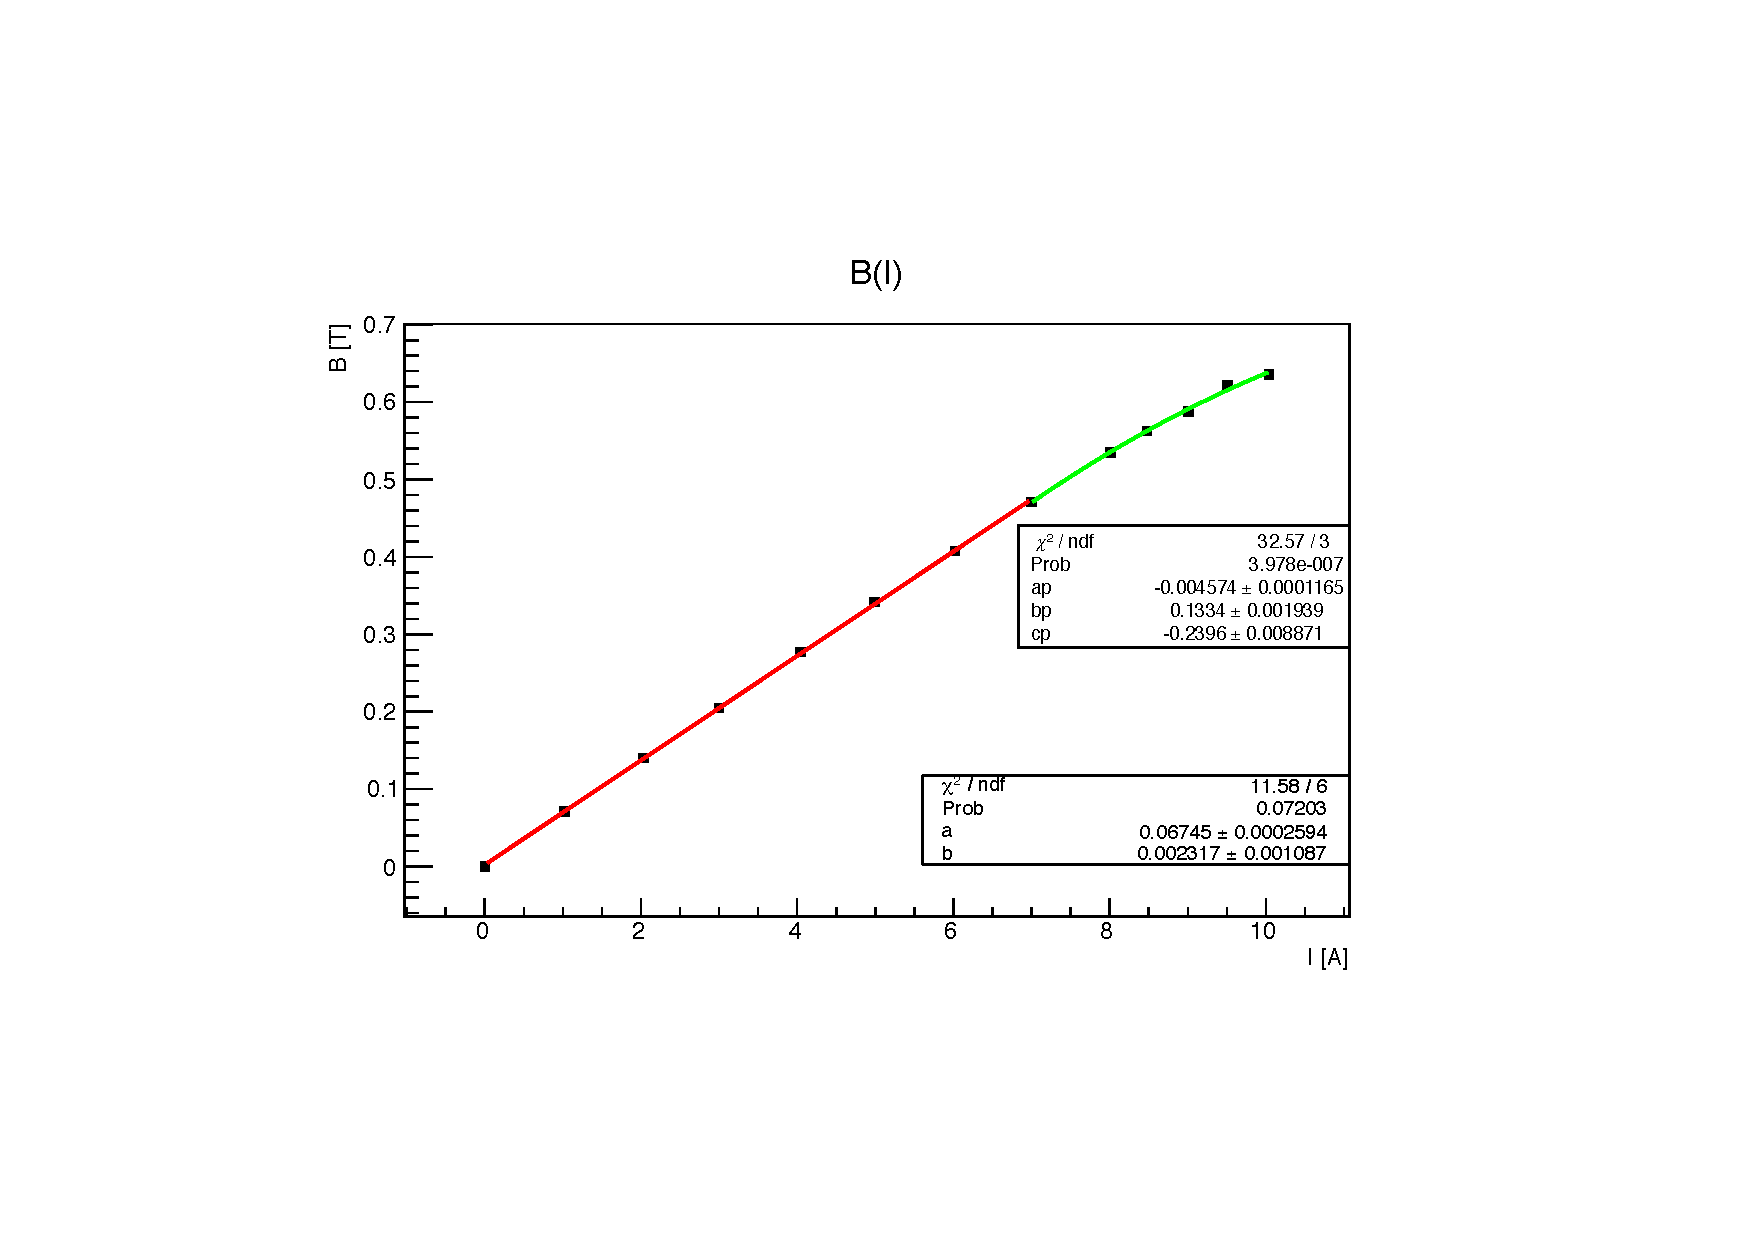
\includegraphics[scale=0.46]{plots/BIcre1.pdf}  &\hspace{0.1cm} 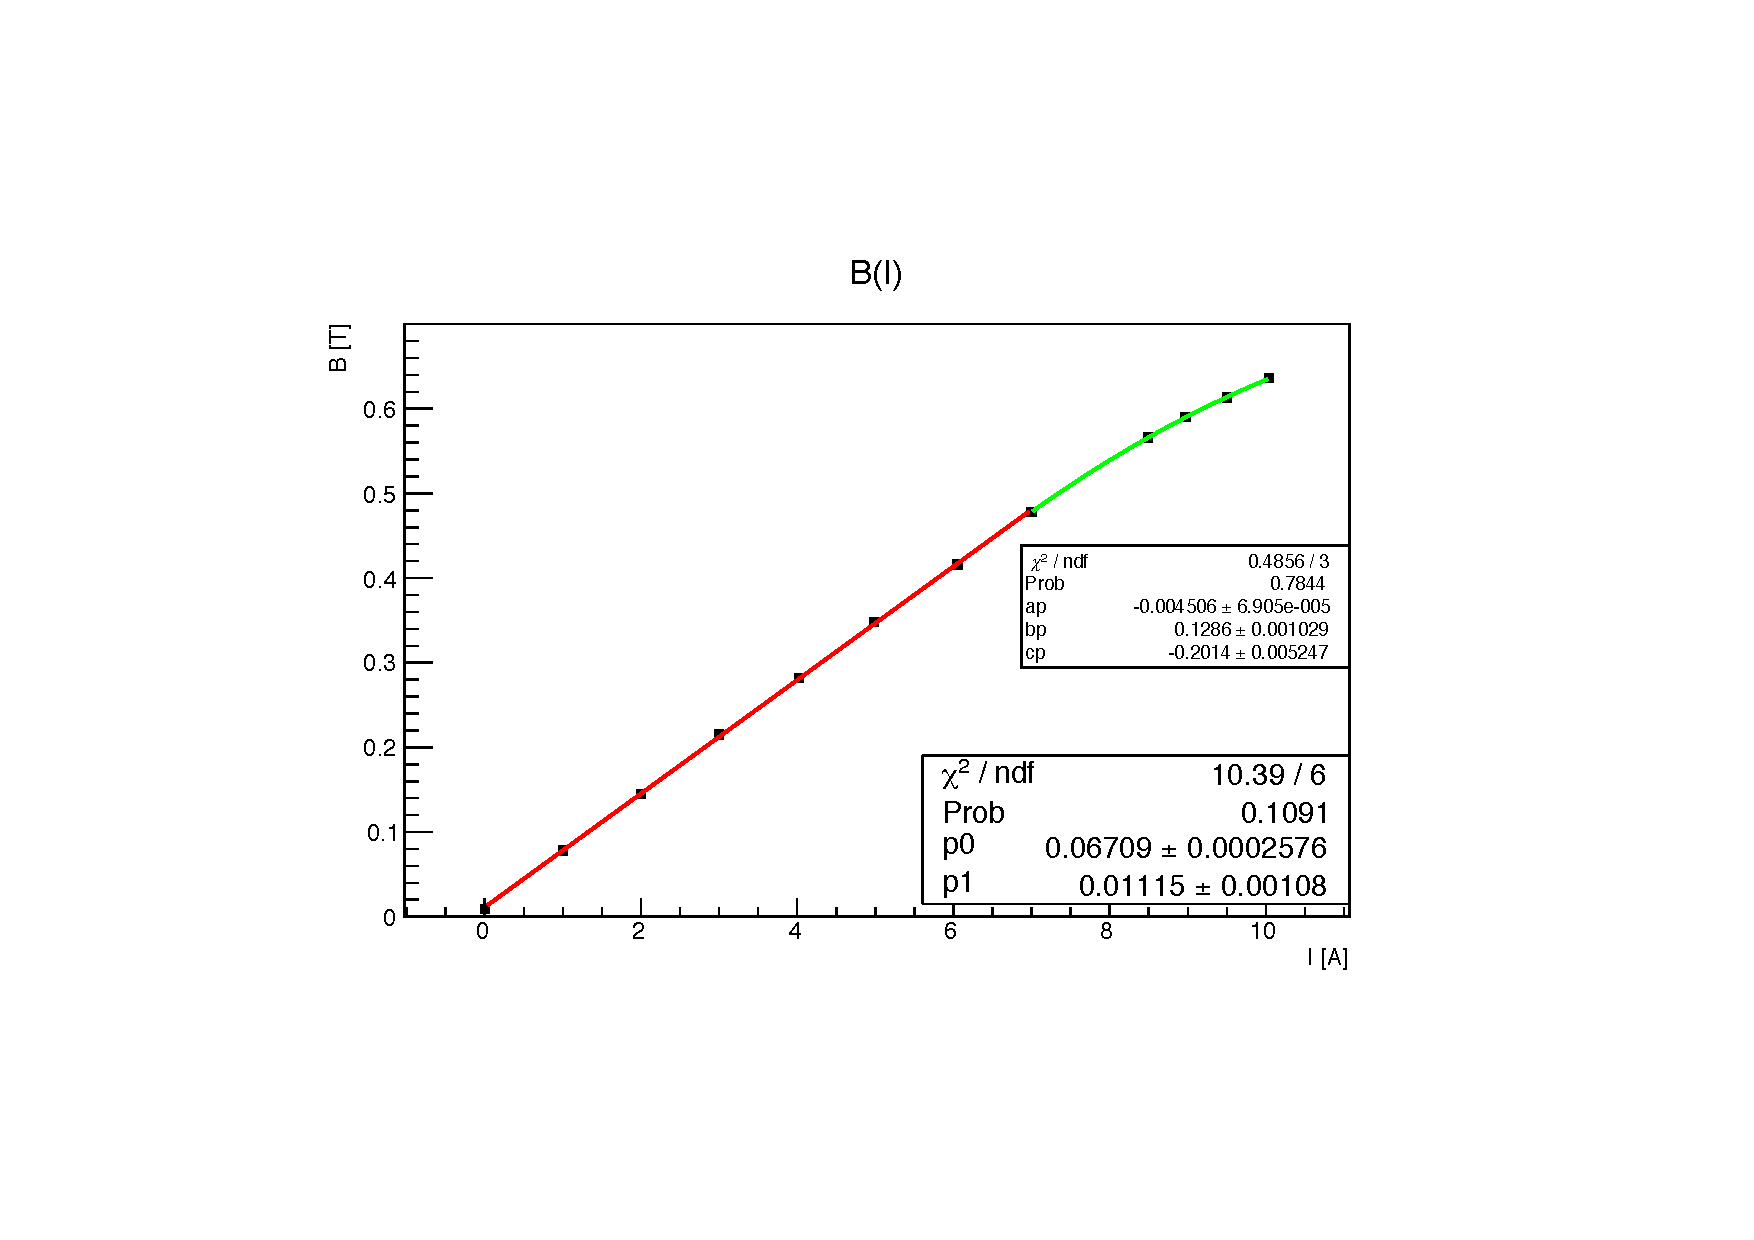
\includegraphics[scale=0.46]{plots/BIdec1.pdf} \\
      \end{tabular}
    \caption{}
    \label{fig:BI1}
\end{figure}
$$
\begin{cases}
f(I)=\boldsymbol{a} I + \boldsymbol{b} \quad \forall I \leq 7.02 \pm 0.02 \text{ A} \\ \\
g(I)= \boldsymbol{a_p}I^2 + \boldsymbol{b_p}I + \boldsymbol{c_p} \quad \forall I > 7.02 \pm 0.02 \text{ A}
\end{cases}
\;\;
\begin{cases}
f(I)=\boldsymbol{p_0} I + \boldsymbol{p_1} \quad \forall I \leq 7.00 \pm 0.02 \text{ A} \\ \\
g(I)= \boldsymbol{a_p}I^2 + \boldsymbol{b_p}I + \boldsymbol{c_p} \quad \forall I > 7.00 \pm 0.02 \text{ A}
\end{cases}
$$

\begin{figure}[H] \hspace{-0.8cm}
    \begin{tabular}{c c}
      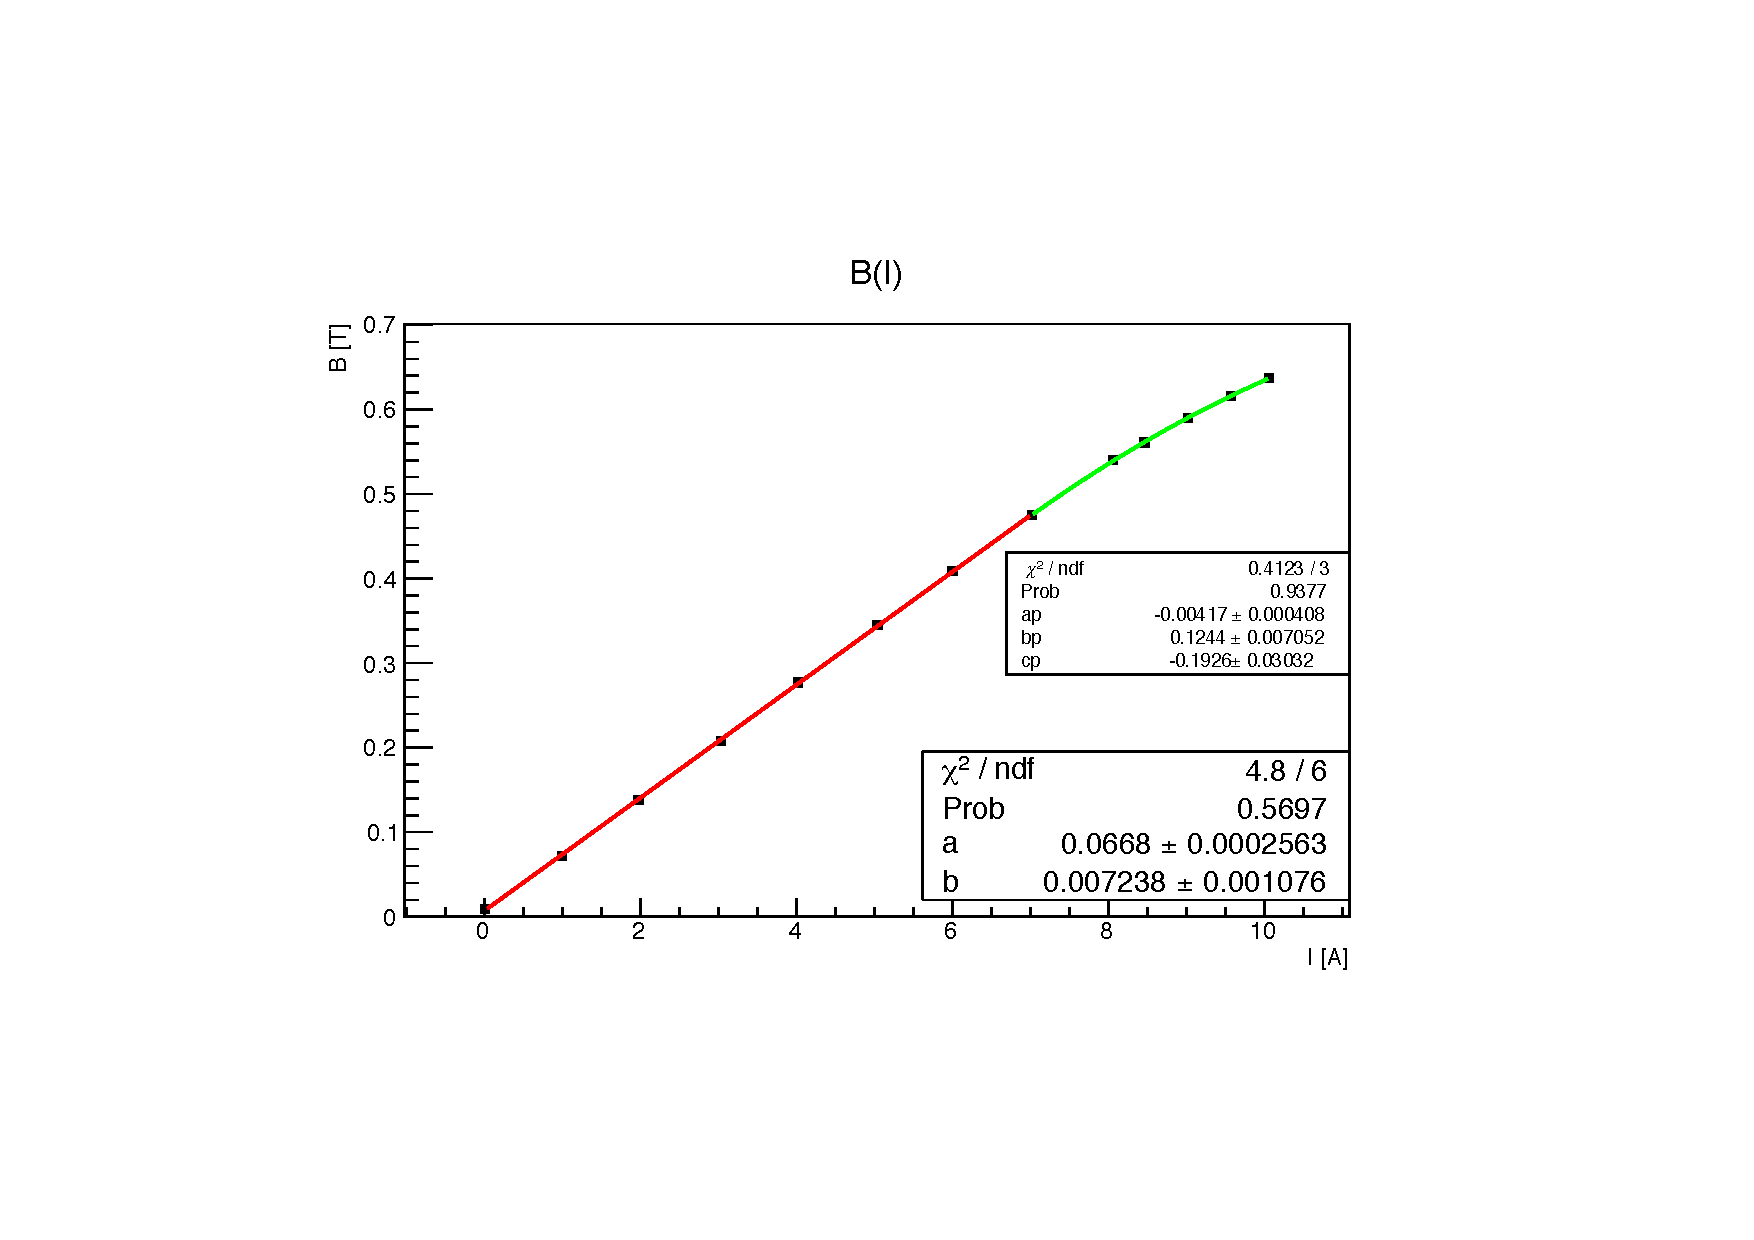
\includegraphics[scale=0.46]{plots/BIcre2.pdf}  &\hspace{0.1cm} 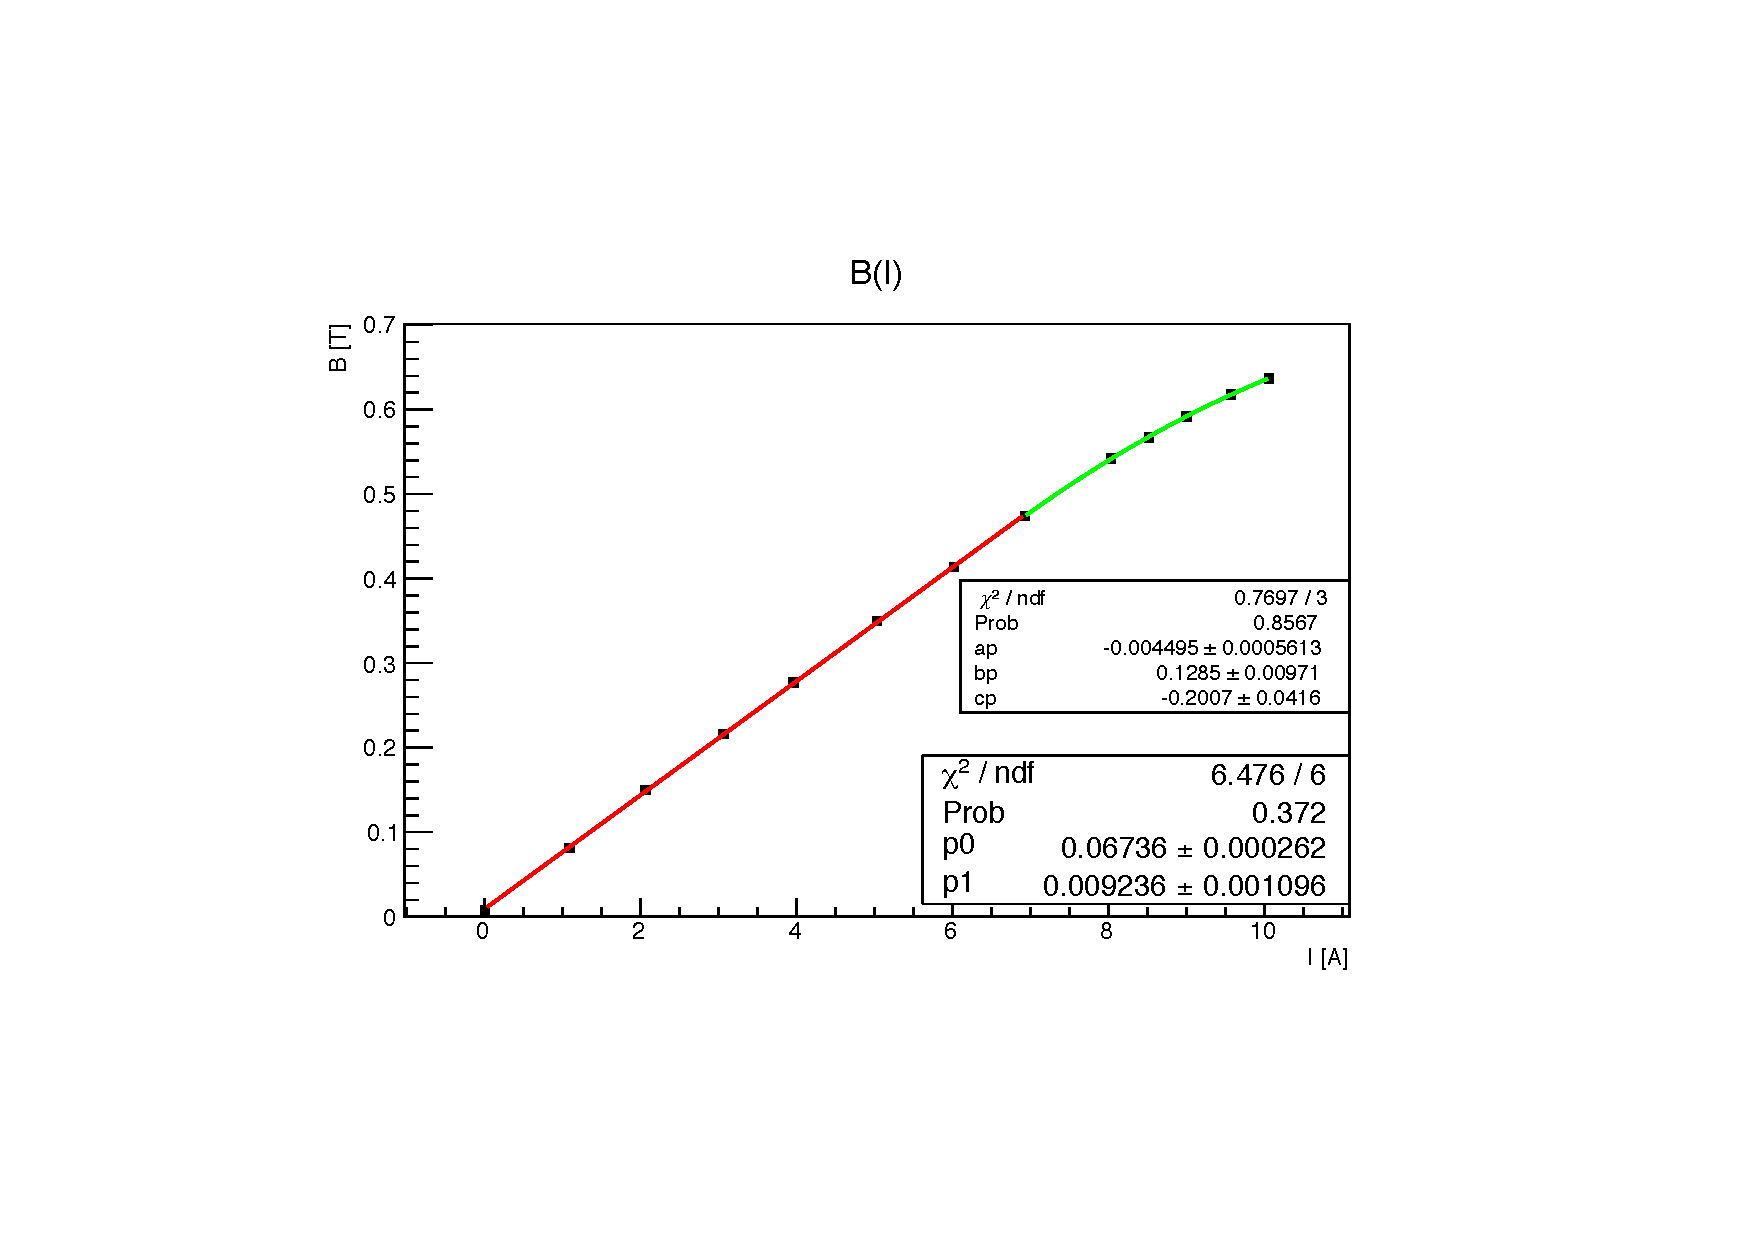
\includegraphics[scale=0.46]{plots/BIdec2.pdf} \\
      \end{tabular}
    \caption{}
    \label{fig:BI2}
\end{figure}
\clearpage
The final calibration curve reported in \hyperref[fig:calcurve]{Figure \ref*{fig:calcurve}} has been calculated as follows: 
\begin{enumerate}
    \item the four values of each parameter have been averaged ;
    \item the compatibility test between every single one with the global average has been computed ;
    \item the compatible ones has been used to get the final curve and their average has been shown to be compatible with the global one.
\end{enumerate}

It might be interesting to observe that, although the magnet we have worked with was a soft ferromagnet, the final calibration curve exhibits a residual magnetization measuring approximately 7 mT . 

\begin{figure}[H]
    \centering
    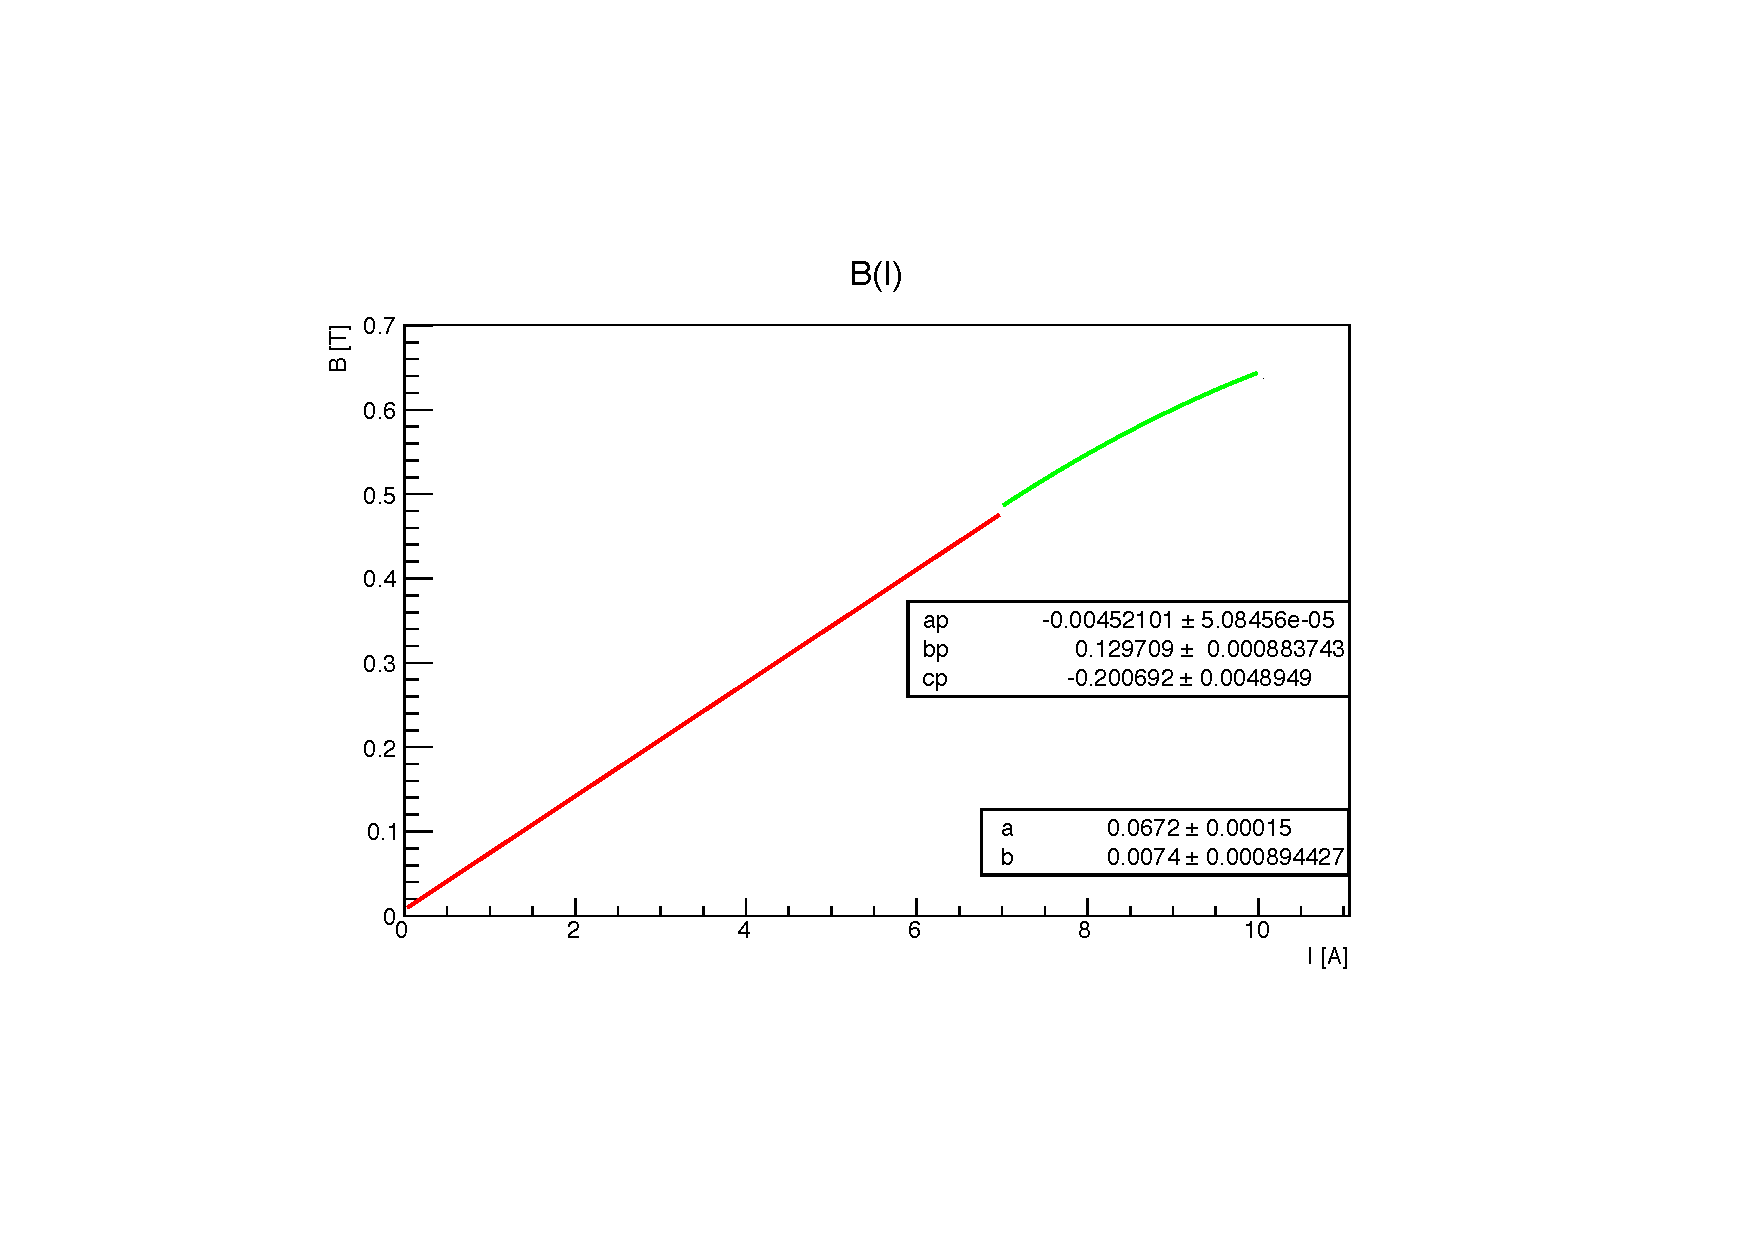
\includegraphics[scale=0.8]{plots/curva.pdf}
    \caption{}
    \label{fig:calcurve}
\end{figure}
From now on the compatibility tests will be evaluated according to the following rules and will never be explicitly stated again in the entire work: 

$$\begin{cases}
Z=\frac{|y-x|}{\sqrt{\delta y^2+ \delta x^2}} \\\\
Z_c = 1.96 \quad(\alpha=0.05) \\\\
\text{Compatibility condition:}\quad Z < Z_c
\end{cases}
$$

\end{document}